% ============================================================
% Question Bank: ch01-06 Applying Proportional Reasoning
% Topic Title: Applying Proportional Reasoning to Real-World Problems
% CCSS: 7.RP.A.2, 7.RP.A.3
% Questions: 30 (18 MC + 7 SA + 5 Graphical)
% ============================================================

% --- Multiple Choice Questions (18) ---

\begin{practiceQuestion}{1-6-q01}{mc}
\begin{questionText}
Five T-shirts cost $\$42.50$. At this rate, how much do $8$ T-shirts cost?
\end{questionText}
\choiceA{$\$56.00$}
\choiceB{$\$64.00$}
\choiceC{$\$68.00$}
\choiceD{$\$72.00$}
\correctAnswer{C}
\explanation{Unit price: $\$42.50 \div 5 = \$8.50$ each. For $8$: $\$8.50 \times 8 = \$68.00$.}
\end{practiceQuestion}

\begin{practiceQuestion}{1-6-q02}{mc}
\begin{questionText}
A map scale says $2$ cm $= 15$ miles. Two cities are $7$ cm apart on the map. What is the actual distance?
\end{questionText}
\choiceA{$42.5$ miles}
\choiceB{$45$ miles}
\choiceC{$52.5$ miles}
\choiceD{$105$ miles}
\correctAnswer{C}
\explanation{Set up a proportion: $\frac{2}{15} = \frac{7}{d}$. Cross-multiply: $2d = 105$, so $d = 52.5$ miles.}
\end{practiceQuestion}

\begin{practiceQuestion}{1-6-q03}{mc}
\begin{questionText}
A car travels $210$ miles on $6$ gallons of gas. How far can it go on $10$ gallons?
\end{questionText}
\choiceA{$300$ miles}
\choiceB{$330$ miles}
\choiceC{$350$ miles}
\choiceD{$360$ miles}
\correctAnswer{C}
\explanation{Unit rate: $210 \div 6 = 35$ mpg. On $10$ gallons: $35 \times 10 = 350$ miles.}
\end{practiceQuestion}

\begin{practiceQuestion}{1-6-q04}{mc}
\begin{questionText}
A recipe for $4$ people uses $\frac{3}{2}$ cups of rice. How much rice is needed for $10$ people?
\end{questionText}
\choiceA{$2\frac{1}{2}$ cups}
\choiceB{$3$ cups}
\choiceC{$3\frac{3}{4}$ cups}
\choiceD{$5$ cups}
\correctAnswer{C}
\explanation{Per person: $\frac{3}{2} \div 4 = \frac{3}{8}$ cup. For $10$: $\frac{3}{8} \times 10 = \frac{30}{8} = 3\frac{3}{4}$ cups.}
\end{practiceQuestion}

\begin{practiceQuestion}{1-6-q05}{mc}
\begin{questionText}
A printer prints $120$ pages in $8$ minutes. How long will it take to print $450$ pages?
\end{questionText}
\choiceA{$25$ min}
\choiceB{$28$ min}
\choiceC{$30$ min}
\choiceD{$36$ min}
\correctAnswer{C}
\explanation{Rate: $120 \div 8 = 15$ pages/min. Time for $450$: $450 \div 15 = 30$ min.}
\end{practiceQuestion}

\begin{practiceQuestion}{1-6-q06}{mc}
\begin{questionText}
Small paint can: $\frac{3}{4}$ gallon for $\$18$. Large can: $1\frac{1}{2}$ gallons for $\$33$. Which is the better buy?
\end{questionText}
\choiceA{Small, at $\$22$/gal}
\choiceB{Large, at $\$22$/gal}
\choiceC{Small, at $\$24$/gal}
\choiceD{Large, at $\$24$/gal}
\correctAnswer{B}
\explanation{Small: $18 \div 0.75 = \$24$/gal. Large: $33 \div 1.5 = \$22$/gal. The large can is $\$2$/gal cheaper.}
\end{practiceQuestion}

\begin{practiceQuestion}{1-6-q07}{mc}
\begin{questionText}
On a map, $3$ cm represents $24$ km. How far apart are two towns that are $8$ cm apart on the map?
\end{questionText}
\choiceA{$48$ km}
\choiceB{$56$ km}
\choiceC{$64$ km}
\choiceD{$72$ km}
\correctAnswer{C}
\explanation{$\frac{3}{24} = \frac{8}{d}$. Cross-multiply: $3d = 192$, so $d = 64$ km.}
\end{practiceQuestion}

\begin{practiceQuestion}{1-6-q08}{mc}
\begin{questionText}
A machine fills $350$ bottles in $5$ hours. How many bottles does it fill in $12$ hours?
\end{questionText}
\choiceA{$700$}
\choiceB{$780$}
\choiceC{$840$}
\choiceD{$900$}
\correctAnswer{C}
\explanation{Rate: $350 \div 5 = 70$ bottles/hr. In $12$ hours: $70 \times 12 = 840$ bottles.}
\end{practiceQuestion}

\begin{practiceQuestion}{1-6-q09}{mc}
\begin{questionText}
Which strategy is NOT a proportional reasoning tool?
\end{questionText}
\choiceA{Find the unit rate and multiply}
\choiceB{Set up a proportion and cross-multiply}
\choiceC{Use $y = kx$}
\choiceD{Add a fixed amount to each value}
\correctAnswer{D}
\explanation{Adding a fixed amount is an additive strategy, not proportional. Proportional strategies use multiplication and division.}
\end{practiceQuestion}

\begin{practiceQuestion}{1-6-q10}{mc}
\begin{questionText}
A recipe uses $2\frac{1}{2}$ cups of flour to make $30$ cookies. How many cups are needed for $48$ cookies?
\end{questionText}
\choiceA{$3$ cups}
\choiceB{$3\frac{1}{2}$ cups}
\choiceC{$4$ cups}
\choiceD{$4\frac{1}{2}$ cups}
\correctAnswer{C}
\explanation{$\frac{2.5}{30} = \frac{x}{48}$. Cross-multiply: $30x = 120$, so $x = 4$ cups.}
\end{practiceQuestion}

\begin{practiceQuestion}{1-6-q11}{mc}
\begin{questionText}
A train travels $315$ miles in $4.5$ hours. At this rate, how far does it travel in $7$ hours?
\end{questionText}
\choiceA{$420$ miles}
\choiceB{$455$ miles}
\choiceC{$490$ miles}
\choiceD{$525$ miles}
\correctAnswer{C}
\explanation{Rate: $315 \div 4.5 = 70$ mph. In $7$ hours: $70 \times 7 = 490$ miles.}
\end{practiceQuestion}

\begin{practiceQuestion}{1-6-q12}{mc}
\begin{questionText}
Store A sells $3$ notebooks for $\$7.50$. Store B sells $5$ notebooks for $\$11.25$. Which store offers the better deal?
\end{questionText}
\choiceA{Store A at $\$2.50$ each}
\choiceB{Store B at $\$2.25$ each}
\choiceC{Store A at $\$2.25$ each}
\choiceD{They cost the same}
\correctAnswer{B}
\explanation{Store A: $7.50 \div 3 = \$2.50$ each. Store B: $11.25 \div 5 = \$2.25$ each. Store B is cheaper.}
\end{practiceQuestion}

\begin{practiceQuestion}{1-6-q13}{mc}
\begin{questionText}
An architect's model uses a scale of $1$ inch $= 3$ feet. If a room in the model is $5.5$ inches long, what is the actual length?
\end{questionText}
\choiceA{$8.5$ feet}
\choiceB{$15$ feet}
\choiceC{$16.5$ feet}
\choiceD{$18$ feet}
\correctAnswer{C}
\explanation{Actual length $= 5.5 \times 3 = 16.5$ feet.}
\end{practiceQuestion}

\begin{practiceQuestion}{1-6-q14}{mc}
\begin{questionText}
A school orders $240$ lunches for $320$ students. At the same rate, how many lunches should they order for $400$ students?
\end{questionText}
\choiceA{$280$}
\choiceB{$300$}
\choiceC{$320$}
\choiceD{$360$}
\correctAnswer{B}
\explanation{$\frac{240}{320} = \frac{x}{400}$. Cross-multiply: $320x = 96{,}000$, so $x = 300$ lunches.}
\end{practiceQuestion}

\begin{practiceQuestion}{1-6-q15}{mc}
\begin{questionText}
A car uses $3$ gallons of gas every $87$ miles. How many gallons does it need for a $435$-mile trip?
\end{questionText}
\choiceA{$10$}
\choiceB{$12$}
\choiceC{$15$}
\choiceD{$18$}
\correctAnswer{C}
\explanation{$\frac{3}{87} = \frac{x}{435}$. Cross-multiply: $87x = 1{,}305$, so $x = 15$ gallons.}
\end{practiceQuestion}

\begin{practiceQuestion}{1-6-q16}{mc}
\begin{questionText}
A factory produces $168$ items in $7$ hours. Another factory produces $200$ items in $8$ hours. Which factory is more productive?
\end{questionText}
\choiceA{Factory 1, at $24$ items/hr}
\choiceB{Factory 2, at $25$ items/hr}
\choiceC{They produce the same rate}
\choiceD{Factory 1, at $25$ items/hr}
\correctAnswer{B}
\explanation{Factory 1: $168 \div 7 = 24$ items/hr. Factory 2: $200 \div 8 = 25$ items/hr. Factory 2 is more productive.}
\end{practiceQuestion}

\begin{practiceQuestion}{1-6-q17}{mc}
\begin{questionText}
A $12$-oz box of cereal costs $\$3.60$. A $20$-oz box costs $\$5.40$. Which is the better value?
\end{questionText}
\choiceA{$12$-oz box at $\$0.30$/oz}
\choiceB{$20$-oz box at $\$0.27$/oz}
\choiceC{$12$-oz box at $\$0.27$/oz}
\choiceD{They are the same price per ounce}
\correctAnswer{B}
\explanation{$12$-oz: $3.60 \div 12 = \$0.30$/oz. $20$-oz: $5.40 \div 20 = \$0.27$/oz. The $20$-oz box is the better value.}
\end{practiceQuestion}

\begin{practiceQuestion}{1-6-q18}{mc}
\begin{questionText}
A painter can paint $3$ rooms in $7$ hours. At this rate, how many hours will it take to paint $9$ rooms?
\end{questionText}
\choiceA{$14$}
\choiceB{$18$}
\choiceC{$21$}
\choiceD{$24$}
\correctAnswer{C}
\explanation{$\frac{3}{7} = \frac{9}{h}$. Cross-multiply: $3h = 63$, so $h = 21$ hours.}
\end{practiceQuestion}

% --- Short Answer Questions (7) ---

\begin{practiceQuestion}{1-6-q19}{sa}
\begin{questionText}
A recipe for $6$ servings uses $\frac{3}{4}$ cup of sugar. How much sugar is needed for $16$ servings?
\end{questionText}
\correctAnswer{$2$ cups}
\explanation{Per serving: $\frac{3}{4} \div 6 = \frac{3}{24} = \frac{1}{8}$ cup. For $16$: $\frac{1}{8} \times 16 = 2$ cups.}
\end{practiceQuestion}

\begin{practiceQuestion}{1-6-q20}{sa}
\begin{questionText}
A cyclist rides $42$ miles in $3$ hours. At this rate, how long does it take to ride $98$ miles?
\end{questionText}
\correctAnswer{$7$ hours}
\explanation{Rate: $42 \div 3 = 14$ mph. Time: $98 \div 14 = 7$ hours.}
\end{practiceQuestion}

\begin{practiceQuestion}{1-6-q21}{sa}
\begin{questionText}
A scale drawing uses $1$ cm $= 4.5$ m. If a building is $27$ m tall, how tall is it in the drawing?
\end{questionText}
\correctAnswer{$6$ cm}
\explanation{$\frac{1}{4.5} = \frac{x}{27}$. Cross-multiply: $4.5x = 27$, so $x = 6$ cm.}
\end{practiceQuestion}

\begin{practiceQuestion}{1-6-q22}{sa}
\begin{questionText}
Brand A juice: $32$ oz for $\$2.56$. Brand B juice: $48$ oz for $\$3.60$. Which brand has the better price per ounce, and what is it?
\end{questionText}
\correctAnswer{Brand B at $\$0.075$ per oz}
\explanation{A: $2.56 \div 32 = \$0.08$/oz. B: $3.60 \div 48 = \$0.075$/oz. Brand B is cheaper per ounce.}
\end{practiceQuestion}

\begin{practiceQuestion}{1-6-q23}{sa}
\begin{questionText}
A garden hose fills a $60$-gallon tank in $8$ minutes. How long does it take to fill a $225$-gallon tank?
\end{questionText}
\correctAnswer{$30$ minutes}
\explanation{Rate: $60 \div 8 = 7.5$ gal/min. Time: $225 \div 7.5 = 30$ minutes.}
\end{practiceQuestion}

\begin{practiceQuestion}{1-6-q24}{sa}
\begin{questionText}
On a map, $4.5$ cm represents $36$ km. Two parks are $54$ km apart. How far apart are they on the map?
\end{questionText}
\correctAnswer{$6.75$ cm}
\explanation{$\frac{4.5}{36} = \frac{x}{54}$. Cross-multiply: $36x = 243$, so $x = 6.75$ cm.}
\end{practiceQuestion}

\begin{practiceQuestion}{1-6-q25}{sa}
\begin{questionText}
A truck delivers $540$ packages in $3$ trips. How many trips are needed to deliver $1{,}620$ packages?
\end{questionText}
\correctAnswer{$9$ trips}
\explanation{Per trip: $540 \div 3 = 180$ packages. Trips needed: $1{,}620 \div 180 = 9$.}
\end{practiceQuestion}

% --- Graphical Questions (3 GMC + 2 GSA) ---

\begin{practiceQuestion}{1-6-q26}{gmc}
\begin{questionText}
The table shows the distance a bus travels over several hours. Using proportional reasoning, how far will the bus travel in $9$ hours?

\begin{center}
\begin{tabular}{|c|c|}
\hline
\textbf{Hours} & \textbf{Miles} \\ \hline
$2$ & $90$ \\ \hline
$5$ & $225$ \\ \hline
$7$ & $315$ \\ \hline
$9$ & $?$ \\ \hline
\end{tabular}
\end{center}
\end{questionText}
\choiceA{$360$ miles}
\choiceB{$385$ miles}
\choiceC{$405$ miles}
\choiceD{$450$ miles}
\correctAnswer{C}
\explanation{Rate: $90 \div 2 = 45$ mph. In $9$ hours: $45 \times 9 = 405$ miles.}
\end{practiceQuestion}

\begin{practiceQuestion}{1-6-q27}{gmc}
\begin{questionText}
A map uses the scale shown below. If two cities are $6.5$ cm apart on the map, what is the actual distance?

\begin{center}
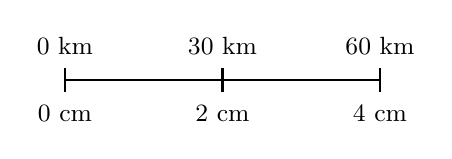
\begin{tikzpicture}[scale=1]
  \draw[thick] (0,0) -- (4,0);
  \draw[thick] (0,-0.15) -- (0,0.15);
  \draw[thick] (2,-0.15) -- (2,0.15);
  \draw[thick] (4,-0.15) -- (4,0.15);
  \node[below] at (0,-0.2) {\small $0$ cm};
  \node[below] at (2,-0.2) {\small $2$ cm};
  \node[below] at (4,-0.2) {\small $4$ cm};
  \node[above] at (0,0.2) {\small $0$ km};
  \node[above] at (2,0.2) {\small $30$ km};
  \node[above] at (4,0.2) {\small $60$ km};
\end{tikzpicture}
\end{center}
\end{questionText}
\choiceA{$90$ km}
\choiceB{$95$ km}
\choiceC{$97.5$ km}
\choiceD{$100$ km}
\correctAnswer{C}
\explanation{Scale: $2$ cm $= 30$ km, so $1$ cm $= 15$ km. For $6.5$ cm: $15 \times 6.5 = 97.5$ km.}
\end{practiceQuestion}

\begin{practiceQuestion}{1-6-q28}{gmc}
\begin{questionText}
The graph below compares the rates of two workers packaging boxes. Which worker is faster, and by how many boxes per hour?

\begin{center}
\begin{tikzpicture}[scale=0.65]
  \draw[step=1,gray!20,thin] (0,0) grid (7,8);
  \draw[thick,->] (0,0) -- (7.5,0) node[right]{\small Hours};
  \draw[thick,->] (0,0) -- (0,8.5) node[above]{\small Boxes};
  \foreach \x in {1,...,7} \draw (\x,0.07) -- (\x,-0.07) node[below]{\tiny \x};
  \foreach \y/\lab in {1/10,2/20,3/30,4/40,5/50,6/60,7/70,8/80}
    \draw (0.07,\y) -- (-0.07,\y) node[left]{\tiny \lab};
  \draw[thick,funBlue] (0,0) -- (6,7.2);
  \fill[funBlue] (0,0) circle (2pt);
  \fill[funBlue] (5,6) circle (2.5pt) node[above left]{\small $(5, 60)$};
  \node[above,funBlue] at (6,7.2) {\small Worker A};
  \draw[thick,funRed] (0,0) -- (6,5.4);
  \fill[funRed] (0,0) circle (2pt);
  \fill[funRed] (5,4.5) circle (2.5pt) node[below right]{\small $(5, 45)$};
  \node[below right,funRed] at (6,5.4) {\small Worker B};
\end{tikzpicture}
\end{center}
\end{questionText}
\choiceA{Worker A, by $3$ boxes/hr}
\choiceB{Worker B, by $3$ boxes/hr}
\choiceC{Worker A, by $15$ boxes/hr}
\choiceD{They work at the same rate}
\correctAnswer{A}
\explanation{Worker A: $60 \div 5 = 12$ boxes/hr. Worker B: $45 \div 5 = 9$ boxes/hr. Worker A is faster by $12 - 9 = 3$ boxes/hr.}
\end{practiceQuestion}

\begin{practiceQuestion}{1-6-q29}{gsa}
\begin{questionText}
The double number line below relates inches on a blueprint to actual feet. A hallway measures $3.5$ inches on the blueprint. What is the actual length?

\begin{center}
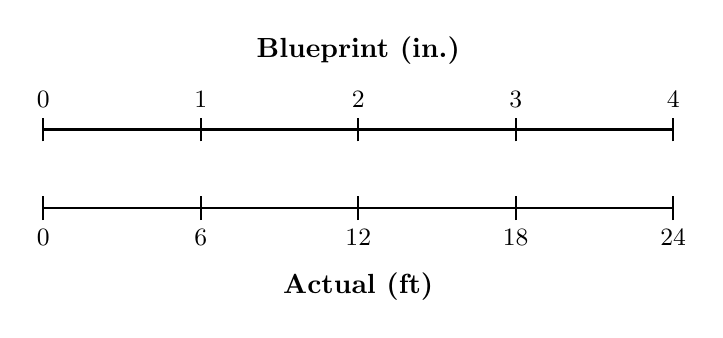
\begin{tikzpicture}[scale=1.0]
  % Top: blueprint inches
  \draw[thick] (0,1) -- (8,1);
  \foreach \x/\lab in {0/$0$, 2/$1$, 4/$2$, 6/$3$, 8/$4$} {
    \draw[thick] (\x,0.85) -- (\x,1.15);
    \node[above] at (\x,1.15) {\small \lab};
  }
  \node[above] at (4,1.7) {\textbf{Blueprint (in.)}};
  % Bottom: actual feet
  \draw[thick] (0,0) -- (8,0);
  \foreach \x/\lab in {0/$0$, 2/$6$, 4/$12$, 6/$18$, 8/$24$} {
    \draw[thick] (\x,-0.15) -- (\x,0.15);
    \node[below] at (\x,-0.15) {\small \lab};
  }
  \node[below] at (4,-0.7) {\textbf{Actual (ft)}};
\end{tikzpicture}
\end{center}
\end{questionText}
\correctAnswer{$21$ feet}
\explanation{Scale: $1$ inch $= 6$ feet. For $3.5$ inches: $6 \times 3.5 = 21$ feet.}
\end{practiceQuestion}

\begin{practiceQuestion}{1-6-q30}{gsa}
\begin{questionText}
The table shows how many batches of muffins a bakery can make and the total flour used. How many cups of flour are needed for $15$ batches?

\begin{center}
\begin{tabular}{|c|c|}
\hline
\textbf{Batches} & \textbf{Flour (cups)} \\ \hline
$3$ & $7\frac{1}{2}$ \\ \hline
$6$ & $15$ \\ \hline
$9$ & $22\frac{1}{2}$ \\ \hline
$15$ & $?$ \\ \hline
\end{tabular}
\end{center}
\end{questionText}
\correctAnswer{$37\frac{1}{2}$ cups}
\explanation{$k = \frac{7.5}{3} = 2.5$ cups per batch. For $15$ batches: $2.5 \times 15 = 37.5 = 37\frac{1}{2}$ cups.}
\end{practiceQuestion}
